\chapter{Auswertung der Ergebnisse}
Im Folgenden werden die unterschiedlichen Fahrstuhl-Scheduler miteinander verglichen. Dazu wurde eine Menge von Fahrstuhl-Rufen zusammengestellt, die im einfachen Scheduler zu einem nahezu konstanten Durchsatz f�hren. Dadurch, dass eine der Metriken konstant ist, sind die Unterschiede zwischen den Metriken der Scheduler deutlicher zu sehen.

F�r die Simulation wurde eine Zeitspanne von 200 Zeiteinheiten festgesetzt. Alle zwei Zeiteinheiten wird ein zuf�lliger Fahrstuhl-Ruf generiert, der vom Scheduler anschlie�end behandelt wird.

\section{Fahrstuhl ohne Kenntnis zuk�nftiger Anfragen}
Im Folgenden werden die ermittelten Werte des einfachen Fahrstuhl-Schedulers dargestellt.

In Diagramm \ref{fig:notknowing_throughput} ist der Durchsatz des einfachen Schedulers dargestellt. Es ist zu sehen, dass der einfache Scheduler nach Ablauf der Simulationszeit 88 Fahrstuhl-Rufe erledigt hat.
\begin{figure}[H]
\centering
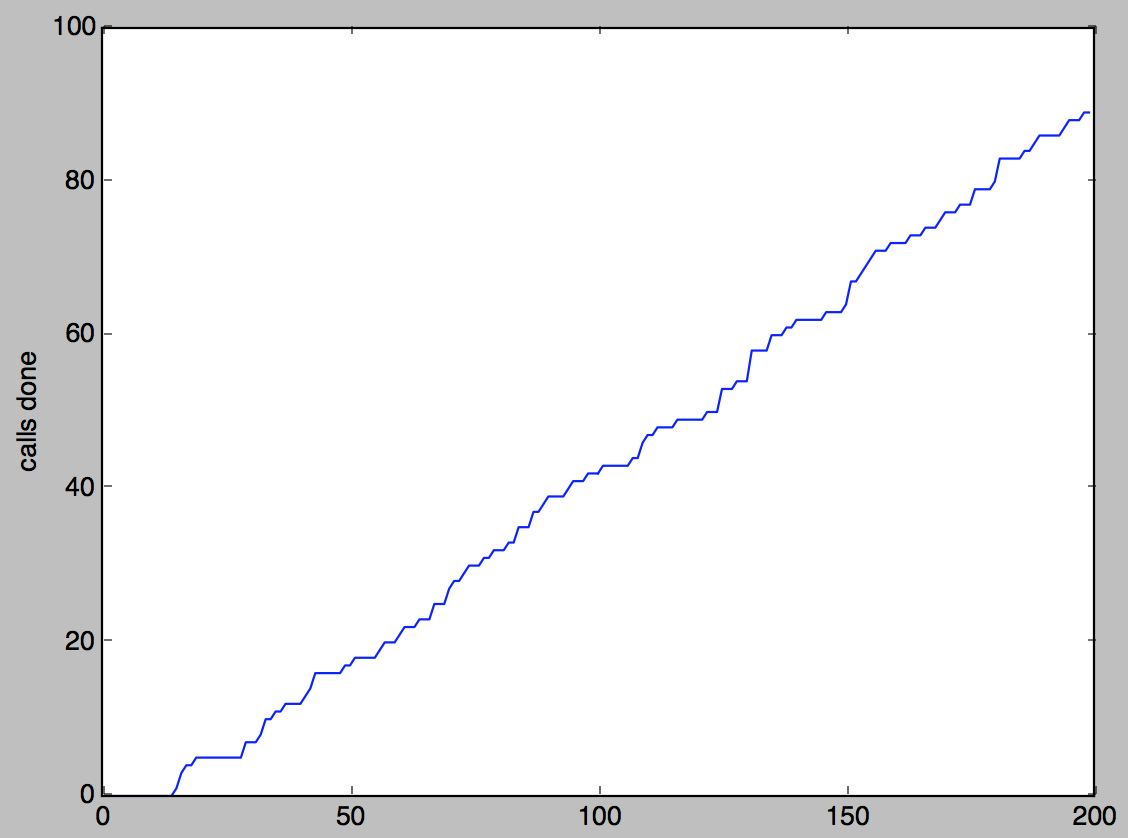
\includegraphics[width=0.5\linewidth]{./NotKnowing_Throughput}
\caption{Durchsatz des einfachen Schedulers}
\label{fig:notknowing_throughput}
\end{figure}

In Abbildung \ref{fig:notknowing_times} sind die durchschnittlichen Warte- und Fahrzeiten pro Zeiteinheit der Fahrstuhlrufe zu sehen.
\begin{figure}[htbp]
	\centering
	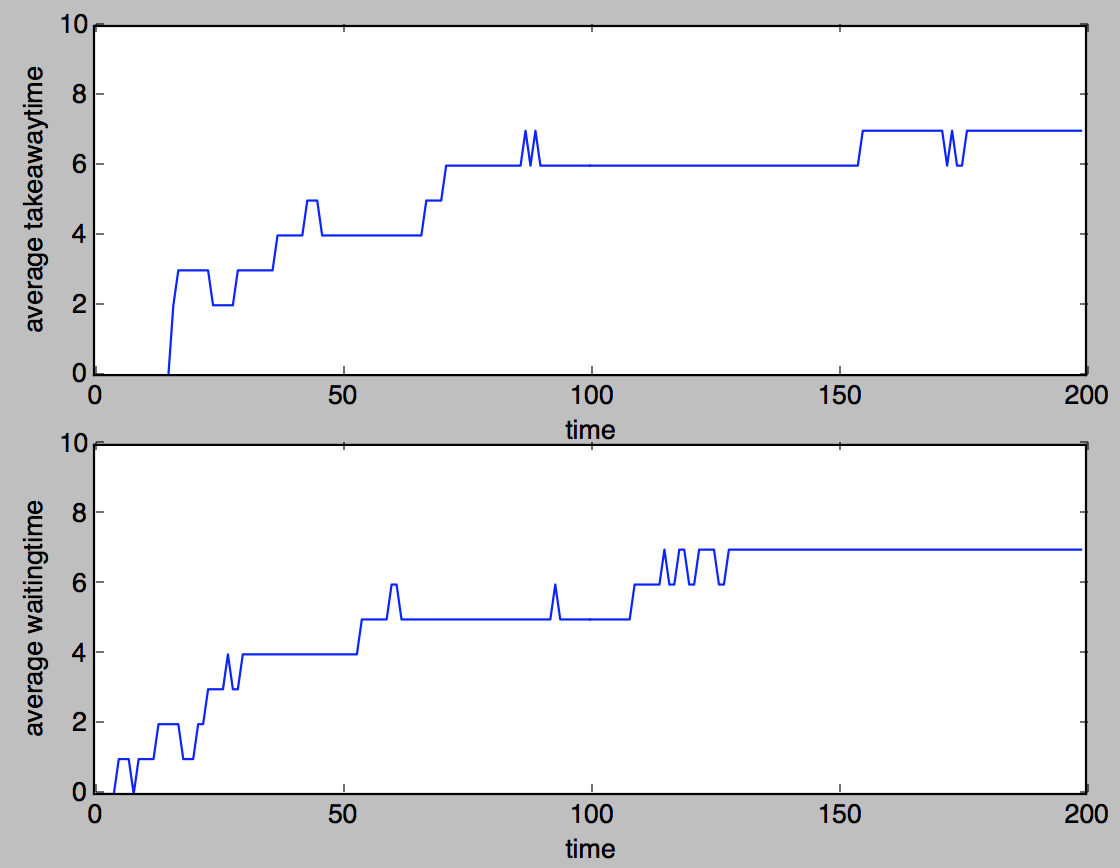
\includegraphics[width=0.7\linewidth]{./NotKnowing_Times}
	\caption{Zeiten des einfachen Schedulers}
	\label{fig:notknowing_times}
\end{figure}


\section{Fahrstuhl mit Kenntnis einiger zuk�nftiger Anfragen}
Im Folgenden werden die ermittelten Werte des wissenden Fahrstuhl-Schedulers dargestellt.

In Diagramm \ref{fig:knowing_throughput} ist der Durchsatz des einfachen Schedulers dargestellt. Es ist zu sehen, dass der wissende Scheduler nach Ablauf der Simulationszeit 92 Fahrstuhl-Rufe erledigt hat.
\begin{figure}[H]
	\centering
	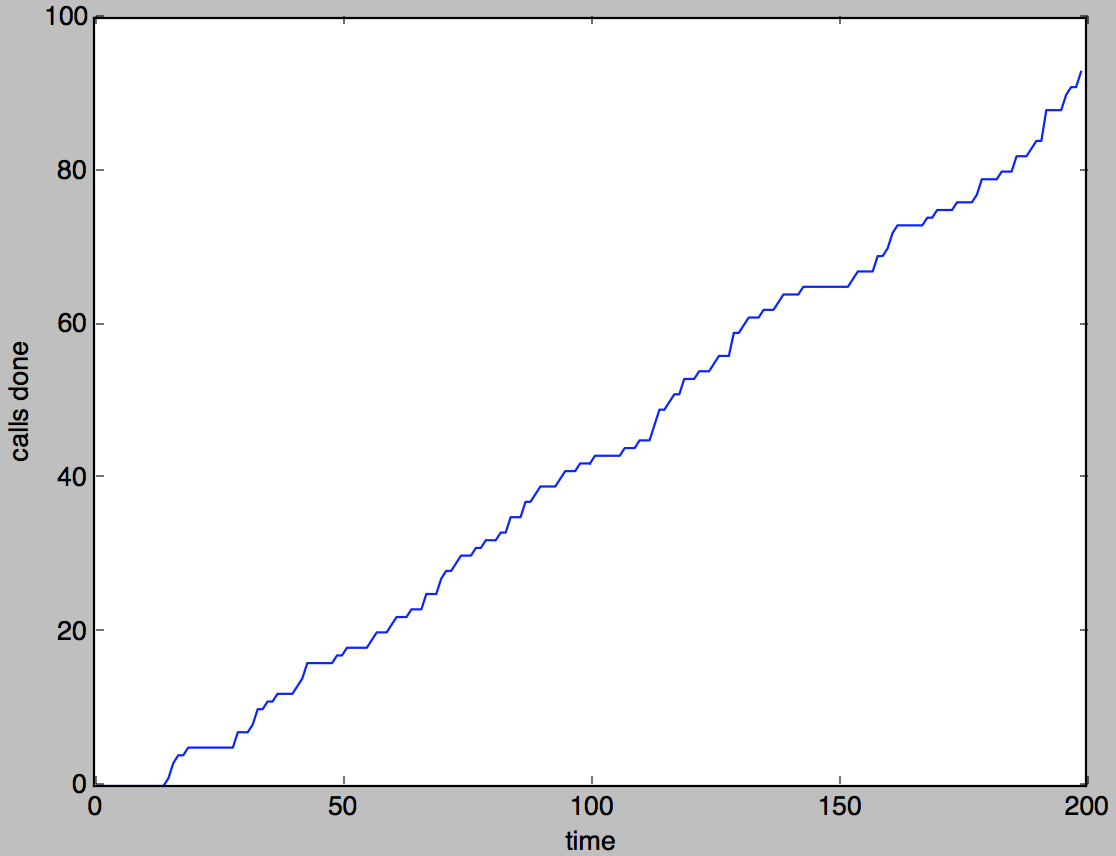
\includegraphics[width=0.5\linewidth]{./Knowing_Throughput}
	\caption{Durchsatz des wissenden Schedulers}
	\label{fig:knowing_throughput}
\end{figure}

In Abbildung \ref{fig:knowing_times} sind die durchschnittlichen Warte- und Fahrzeiten pro Zeiteinheit der Fahrstuhlrufe zu sehen.
\begin{figure}[htbp]
	\centering
	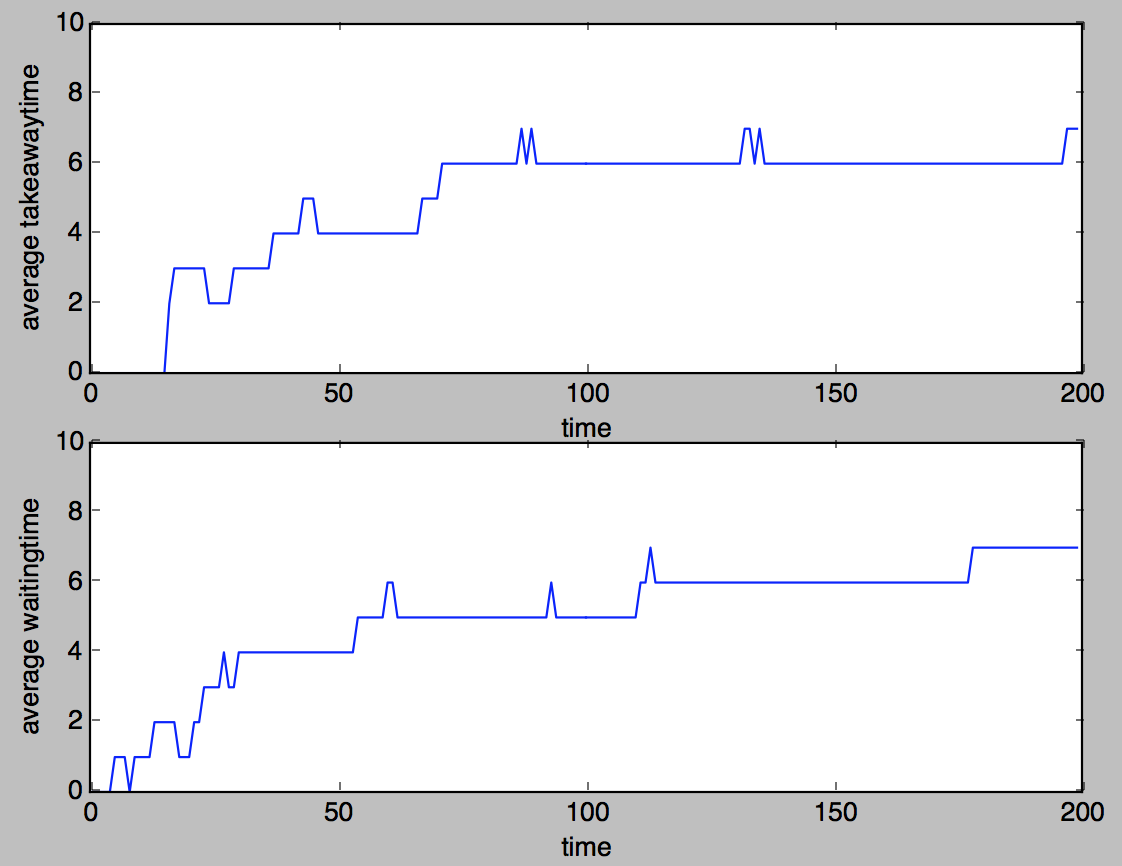
\includegraphics[width=0.7\linewidth]{./Knowing_Times}
	\caption{Zeiten des wissenden Schedulers}
	\label{fig:knowing_times}
\end{figure}

\section{Betrachtung einzelner Anfragen}
Einige zuf�llig ausgew�hlte Fahrstuhl-Anfragen wurden in der Simulation so konfiguriert, dass sie dem wissenden Scheduler vorzeitig bekannt sind. F�r diese dedizierten Anfragen wurden einige Werte erfasst, die im Folgenden gezeigt werden. Dort ist au�erdem zu sehen, zu welchem Zeitpunkt die Anfrage in das Scheduling des Schedulers eingegangen ist. Dieser Zeitpunkt ist in der Tabelle \ref{table:request_times} in der Spalte \textit{Scheduler-Zeit} gef�hrt.

Die Zeitwerte sind in der Tabelle \ref{table:request_times} aufgef�hrt. Die Zeit-Werte einer Zelle sind dabei folgenderma�en zu lesen:
\textit{a/b} wobei \textit{a} der Wert ist, der im einfachen Scheduler erreicht wurde und \textit{b} der Wert ist, der im wissenden Scheduler erreicht wurde.

\begin{table}[H]
\centering
\begin{tabular}{c|c|c|c}
ID der Anfrage & Scheduler-Zeit & Wartezeit & Fahrzeit \\ 
\hline 
52 & 104/94 & 115/105 & 131/119 \\ 
\hline 
59 & 118/108 & 134/129 & 140/135 \\ 
\hline 
74 & 148/138 & 163/149 & 176/158 \\ 
\hline 
83 & 166/156 & 166/167 & 169/170 \\ 
\end{tabular}
\caption{Zeit-Werte von ausgew�hlten Anfragen}
\label{table:request_times}
\end{table}

\section{Analyse}
Nimmt man die Abbildungen dieses Kapitels f�r sich, haben sie keine Aussagekraft. Im Folgenden werden sie miteinander verglichen, um einen Wert aus ihnen zu ziehen.

Vergleicht man die Durchsatz-Abbildungen, dann sieht man, dass der wissende Scheduler einige Fahrstuhlrufe mehr beendet hat als der einfache Scheduler. Dies ist auf die Konstellation der zuf�llig erstellen Fahrstuhlrufe zur�ckzuf�hren und ist f�r diese Betrachtung nicht von Interesse. Simulationen mit anderen zuf�lligen Fahrstuhlruf-Konstellationen hat gezeigt, dass der einfache Scheduler ebenso einen h�heren Durchsatz erreichen kann als der wissende Scheduler.

Was au�erdem auff�llt ist, dass die Kurve anders verl�uft. Bis zum Zeitpunk 104 verlaufen die Durchsatz-Kurven der beiden Scheduler gleichm��ig. Zu dem Zeitpunkt tritt der erste zuk�nftige Fahrstuhlruf auf. Man sieht in den Graphen, dass in der Kurve des wissenden Scheduler - im Vergleich zum einfachen Scheduler - an dieser Stelle weniger Rufe erledigt wurden. Dies liegt am ver�nderten Scheduling-Verhalten, das in in Abschnitt \ref{sec:model} erkl�rt wird. An den Zeitpunkten 118, 148 und 166 treten ebenfalls zuk�nftige Rufe auf. Zu diesen Zeitpunkten ist ebenfalls niedriges Wachstum in Abbildung \ref{fig:knowing_throughput} zu finden.

�hnlich ist es in den Zeit-Graphen (Abbildungen \ref{fig:notknowing_times} und \ref{fig:knowing_times}). Auch dort verlaufen die Kurven der beiden Scheduler bis zum Auftreten des ersten zuk�nftigen Fahrstuhlrufs deckungsgleich. Ab dem Zeitpunkt 104 verl�uft die Kurve des wissenden Schedulers anders als die des einfachen Schedulers. Die Durchschnittswerte der Warte- und Fahrzeiten des einfachen Schedulers wachsen nach dem Zeitpunkt 104 auf den Wert sieben an. Dieses Wachstum gibt es beim wissenden Schedulers auch, dort erfolgt das Wachstum allerdings erst sp�ter. Diese Wachstums-Verz�gerung ist nicht von Bedeutung, denn Simulationsversuche mit anderen zuf�lligen Fahrstuhlruf-Konstellationen haben gezeigt, dass der wissende Scheduler ebenso deutlich h�here Zeit-Werte als der einfache Scheduler erreichen kann.



